\documentclass[
  bibliography=totoc,     % Literatur im Inhaltsverzeichnis
  captions=tableheading,  % Tabellenüberschriften
  titlepage=firstiscover, % Titelseite ist Deckblatt
  parskip=half, % !!! halbzeiliger vertikaler Abstand (siehe Latex-Skript S.125)
]{scrartcl}

% !!! Python in Latex
\usepackage{pythontex}

% !!! zum Drehen von Seiten
\usepackage{adjustbox}

% Paket float verbessern
\usepackage{scrhack}

% Warnung, falls nochmal kompiliert werden muss
\usepackage[aux]{rerunfilecheck}

% unverzichtbare Mathe-Befehle
\usepackage{amsmath}
% viele Mathe-Symbole
\usepackage{amssymb}
% Erweiterungen für amsmath
\usepackage{mathtools}

% Fonteinstellungen
\usepackage{fontspec}
% Latin Modern Fonts werden automatisch geladen
% Alternativ zum Beispiel:
%\setromanfont{Libertinus Serif}
%\setsansfont{Libertinus Sans}
%\setmonofont{Libertinus Mono}

% Wenn man andere Schriftarten gesetzt hat,
% sollte man das Seiten-Layout neu berechnen lassen
\recalctypearea{}

% deutsche Spracheinstellungen
\usepackage[ngerman]{babel}

% !!! babel mit anderen Sprachen laden für \enquote (siehe latex-Skript S.33)
\usepackage[autostyle]{csquotes}

% !!! zum durchstreichen durch \cancel{}
\usepackage[makeroom]{cancel}

% !!! zum Ersetzen von \symup{} durch z.B. \dif{} (siehe latex-Skript)
\usepackage{expl3}
\usepackage{xparse}
\ExplSyntaxOn
\NewDocumentCommand \dif {m} {
  \mathinner{\symup{d} #1}
}
\ExplSyntaxOff

% !!! Nummerierung von Gleichungen nach Sections: Bei langen Dokumenten empfohlen
% \numberwithin{equation}{section}


\usepackage[
  math-style=ISO,    % ┐
  bold-style=ISO,    % │
  sans-style=italic, % │ ISO-Standard folgen
  nabla=upright,     % │
  partial=upright,   % ┘
  warnings-off={           % ┐
    mathtools-colon,       % │ unnötige Warnungen ausschalten
    mathtools-overbracket, % │
  },                       % ┘
]{unicode-math}

% traditionelle Fonts für Mathematik
\setmathfont{Latin Modern Math}
% Alternativ zum Beispiel:
%\setmathfont{Libertinus Math}

\setmathfont{XITS Math}[range={scr, bfscr}]
\setmathfont{XITS Math}[range={cal, bfcal}, StylisticSet=1]

% Zahlen und Einheiten
\usepackage[
  locale=DE,                   % deutsche Einstellungen
  separate-uncertainty=true,   % immer Unsicherheit mit \pm
  per-mode=symbol-or-fraction, % / in inline math, fraction in display math
]{siunitx}

% chemische Formeln
\usepackage[
  version=4,
  math-greek=default, % ┐ mit unicode-math zusammenarbeiten
  text-greek=default, % ┘
]{mhchem}

% richtige Anführungszeichen
\usepackage[autostyle]{csquotes}

% schöne Brüche im Text
\usepackage{xfrac}

% Standardplatzierung für Floats einstellen
\usepackage{float}
\floatplacement{figure}{htbp}
\floatplacement{table}{htbp}

% Floats innerhalb einer Section halten
\usepackage[
  section, % Floats innerhalb der Section halten
  below,   % unterhalb der Section aber auf der selben Seite ist ok
]{placeins}

% Seite drehen für breite Tabellen: landscape Umgebung
\usepackage{pdflscape}

% Captions schöner machen.
\usepackage[
  labelfont=bf,        % Tabelle x: Abbildung y: ist jetzt fett
  font=small,          % Schrift etwas kleiner als Dokument
  width=0.9\textwidth, % maximale Breite einer Caption schmaler
]{caption}

% subfigure, subtable, subref
\usepackage{subcaption}

% Grafiken können eingebunden werden
\usepackage{graphicx}

% !!! Textumflossene Grafiken
\usepackage{wrapfig}

% !!! Kreisnummern
\usepackage{tikz} 

% !!! größeres Seitenlayout für mehr Platz
\usepackage[a4paper, left=30mm, top=30mm, right=30mm, bottom=40mm]{geometry} 

% !!! Aufgaben nummerieren
\usepackage{tasks}

% !!! Für das Einfügen von pdfs wie Messdaten etc.
\usepackage{pdfpages}

% schöne Tabellen
\usepackage{booktabs}

% Verbesserungen am Schriftbild
\usepackage{microtype}

% Literaturverzeichnis
\usepackage[
  backend=biber,
]{biblatex}
% Quellendatenbank
\addbibresource{lit.bib}
\addbibresource{programme.bib}

% Hyperlinks im Dokument
\usepackage[
  german,
  unicode,        % Unicode in PDF-Attributen erlauben
  pdfusetitle,    % Titel, Autoren und Datum als PDF-Attribute
  pdfcreator={},  % ┐ PDF-Attribute säubern
  pdfproducer={}, % ┘
]{hyperref}
% erweiterte Bookmarks im PDF
\usepackage{bookmark}

% Trennung von Wörtern mit Strichen
\usepackage[shortcuts]{extdash}

\author{%
  AUTOR A\\%
  \href{mailto:authorA@udo.edu}{authorA@udo.edu}%
  \and%
  AUTOR B\\%
  \href{mailto:authorB@udo.edu}{authorB@udo.edu}%
}
\publishers{TU Dortmund – Fakultät Physik}
\setlength\parindent{0pt}

\subject{V503}
\title{Der Millikan-Öltröpfchenversuch}
\date{
  Durchführung: 13.12.2022
  \hspace{3em}
  Abgabe: 20.12.2022
}
\author{Katharina Kürschner \and Leonard Trinschek}

\begin{document}

\maketitle
\thispagestyle{empty}
\tableofcontents
\newpage

\section{Ziel}
Ziel dieses Versuches ist die Bestimmung der 
Elementarladung mithilfe einer leicht abgewandelten 
Version der Millikan Methode.
\label{sec:Ziel}




\section{Theorie}
\label{sec:Theorie}

Die Milikan-Methode zur Bestimmung der Elementarladung basiert auf der Zerstäubung von Öltröpfchen in das elektrische Feld eines Plattenkondensators. 
Durch die Reibung der Tröpfchen mit der Luft werden sie elektrisch geladen. Die Ladung $q$ der Tröpfchen kann nur ein ganzzahliges Vielfaches der 
Elementarladung sein. Das elektrische Feld des Plattenkondensators ist vertikal ausgerichtet, wodurch die auf die geladenen Teilchen wirkende 
elektrische Kraft $\vec{F}_\text{el}$ parallel oder antiparallel zur Gravitationskraft $\vec{F}_\text{g}$ wirkt. Zusätzlich wirkt die Stokesche 
Reibungskraft $\vec{F}_\text{R}$ entgegen der Bewegungsrichtung, da sich die Teilchen mit einer Geschwindigkeit $\vec{v}$ durch den luftgefüllten 
Raum bewegen.

Die Wirkung dieser Kräfte auf ein Teilchen kann durch folgende Gleichungen beschrieben werden:

\begin{align}
    \label{eqn:Kraefte}
    \vec{F}_\text{g} &= m \vec{g} \\
    \vec{F}_\text{el} &= q \vec{E} \\
    \vec{F}_\text{R} &= -6\symup{\pi}r\eta_\text{L} \vec{v}
\end{align}

Hierbei steht $m$ für die Masse des Teilchens, $\vec{g}$ für die Fallbeschleunigung, $\eta_\text{L}$ für die Viskosität der Luft und $r$ für den Radius 
des Teilchens.

Nach einer kurzen Zeit stellt sich ein Kräftegleichgewicht ein, bei dem sich die Tröpfchen mit konstanter Geschwindigkeit bewegen. Bei abgeschaltetem 
elektrischen Feld bewegen sich die Öltröpfchen mit der Geschwindigkeit $v_0$ und erhalten durch den Auftrieb der Luft den Radius:

\begin{equation}
    \label{eqn:Radius}
    r = \sqrt{\frac{9 \eta_\text{L}(v_\text{ab} - v_\text{auf})}{4g(\rho_\text{Oel}- \rho_\text{L})}}.
\end{equation}

Das Kräftegleichgewicht führt zu folgender Gleichung:

\begin{equation*}
    \frac{4\symup{\pi}}{3}r^3(\rho_\text{Oel}- \rho_\text{L})g = 6 \symup{\pi} \eta_\text{L}r v_0.
\end{equation*}

Abhängig von der Polung des elektrischen Feldes wirken die elektrostatische Kraft und die Reibungskraft in verschiedene Richtungen. Die Orientierung 
der Kräfte kann der Abbildung \ref{fig:Kraeftegleichgewicht} entnommen werden.

\begin{figure}
    \centering
    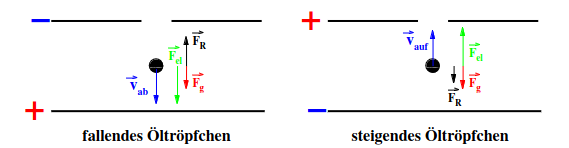
\includegraphics[width = .9\textwidth]{Bilder/Kraeftegleichgewicht.png}
    \caption{Orientierung der wirkenden Kräfte bei unterschiedlicher Polung des elektrischen Feldes. \cite{1}}
    \label{fig:Kraeftegleichgewicht}
\end{figure}

Wenn die obere Platte des Kondensators positiv geladen ist und eine ausreichend große Spannung anliegt, bewegt sich das Öltröpfchen mit der 
Geschwindigkeit $v_\text{auf}$ nach oben. Das Kräftegleichgewicht ergibt sich zu:

\begin{equation*}
    \label{eqn:Kraefte_1}
    \frac{4\symup{\pi}}{3}r^3(\rho_\text{Oel} - \rho_\text{L})g + 6 \symup{\pi} \eta_\text{L}r v_\text{auf} = qE.
\end{equation*}

Bei entgegengesetzter Polung des elektrischen Feldes ergibt sich:

\begin{equation*}
    \label{eqn:Kraefte_2}
    \frac{4\symup{\pi}}{3}r^3(\rho_\text{Oel}- \rho_\text{L})g - 6 \symup{\pi} \eta_\text{L}r v_{\text{ab}} = -qE,
\end{equation*}

wobei $v_{\text{ab}}$ die nach unten gerichtete Geschwindigkeit ist.

Aus diesen beiden Gleichungen kann die Ladung $q$ des Öltröpfchens bestimmt werden:

\begin{equation}
    \label{eqn:q}
    q = \frac{9}{2} \symup{\pi} \sqrt{\frac{\eta_\text{L}^3(v_\text{ab} - v_\text{auf})}{g(\rho_\text{Oel}- \rho_\text{L})}} \cdot \frac{v_\text{ab} + v_\text{auf}}{E},
\end{equation}

wobei $E$ den Betrag des elektrischen Feldes darstellt. Die Geschwindigkeiten sind durch folgenden Zusammenhang gegeben:

\begin{equation}
    \label{eqn:v_0}
    2v_0 = v_\text{ab} - v_\text{auf}.
\end{equation}

Bei diesen Gleichungen \ref{eqn:q} muss eine Korrektur durchgeführt werden, weil die Gleichungen nur für Tröpfchen gelten deren Abmessungen größer 
als die mittlere freie Weglänge in Luft ist.
Die Korrektur ist dabei gegeben als
\begin{align}
\label{eq:Theorie_Cunningham_Viskositaet}
\eta_\text{eff}=\eta_\text{L}\left( \frac{1}{1+B\frac{1}{pr}} \right),
\end{align}
sie wird als \textbf{Cunningham-Korrekturterm} bezeichnet. 
Dazu wird der Luftdruck $p$ und die experimentell bestimmbare Konstante $B =  \num{6.17e-3}\, \text{Torr}\cdot\unit{\centi\metre}$ \cite{1} verwendet.
Es gilt $1\,\text{Torr} \approx \qty{133.322}{\pascal}$ \cite{2}.
Für die korrigierte Ladung gilt
\begin{equation}
    \label{eqn:q_korrigiert}
    q_\text{real} = q_0 \left(1+ \frac{B}{pr}\right)^{-3/2}.
\end{equation}
\section{Versuchsaufbau und Durchführung}
\label{sec:Durchführung}

\subsection{Versuchsaufbau}
\label{subsec:Versuchsaufbau}
Der Versuchsaufbau besteht aus einer Kammer mit einem Plattenkondensator, der eine kleine Öffnung an der Oberseite aufweist. 
Diese Oberseite wird zum Einspritzen von zerstäubten Öltröpfchen verwendet. Die Platten des Kondensators haben einen Abstand 
von $d = (7,6250 \pm 0,0051) \, \si{\milli\meter}$.

Um die Tröpfchen gut sichtbar zu machen, werden sie seitlich von einer Halogenlampe beleuchtet. Die Temperatur der Luft in der 
Kammer wird mit einem Thermowiderstand kontrolliert, dessen Wert an einem Multimeter abgelesen werden kann. Ebenso kann die 
Spannung zwischen den beiden Kondensatorplatten an einem Multimeter abgelesen werden.

Durch das Zerstäuben sind die meisten Öltröpfchen geladen, während einige nicht geladen sind. Die nicht geladenen Tröpfchen 
können durch ein schwach radioaktives $\alpha$-Präparat ionisiert werden. Durch einen Schalter kann das Präparat abgeschirmt 
oder aktiviert werden.

Die Polung der Kondensatorplatten kann mit einem Schalter geändert werden. Mit einer Libelle kann überprüft und eingestellt 
werden, ob die Apparatur gerade steht. Die Tröpfchen können mit einem Mikroskop beobachtet werden.

Der Versuchsaufbau ist in Abbildung \ref{fig:Versuchsaufbau} dargestellt.

\begin{figure}[H]
    \centering
    \caption{Schematischer Aufbau der Versuchsappartatur zum Millikan-Öltröpchen-Versuch.\cite{1}}
    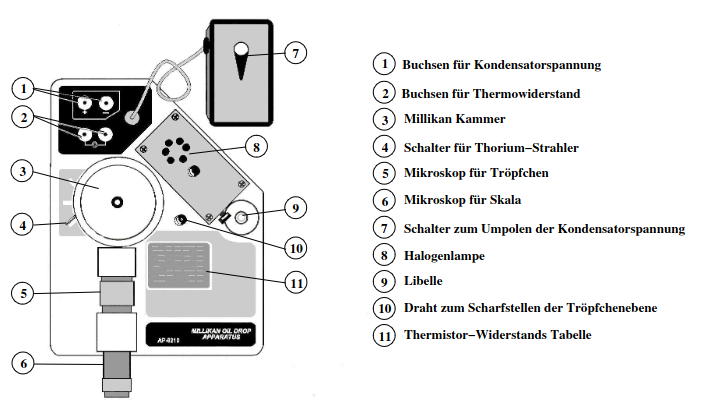
\includegraphics[width=\textwidth]{Bilder/Versuchsaufbau.png}
    \label{fig:Versuchsaufbau}
\end{figure}


\subsection{Durchführung}
\label{subsec:Durchführung}

Zu Beginn wird die Ausrichtung der Apparatur überprüft, um sicherzustellen, dass sie waagerecht steht. Dies wird mithilfe einer 
Libelle durchgeführt.Außerdem wird durch fokussieren auf eine Nadelspitze die Linse eingestellt.
Anschließend werden die Kondensatorplatten geerdet und Öltröpfchen in die Kammer eingesprüht. Während des 
Einsprühens wird mithilfe eines Mikroskops überwacht, wie viele Tröpfchen in die Kammer gelangen.

Nun werden bei zwei verschiedenen Spannungen 22 verschiedene Tröpfchen beobachtet. Dabei werden die Zeiten für den Aufstieg 
und den Abstieg eines Tröpfchens über eine festgelegte Strecke jeweils drei Mal gemessen. Vor jeder Messung wird der Wert 
der Temperatur für jedes Tröpfchen erfasst.

Die verwendeten Spannungen betragen 200 V und 230 V. Durch das Umpolen mithilfe des Schalters werden die Tröpfchen entweder 
in Aufwärts- oder Abwärtsbewegung gebracht.



\section{Fehlerrechnung}
\label{sec:Fehlerrechnung}
Für die Fehlerrechnung werden folgende Formeln aus der Vorlesung verwendet.
Für den Mittelwert gilt
\begin{equation}
    \overline{x}=\frac{1}{N}\sum_{i=1}^N x_i ß\; \;\text{mit der Anzahl N und den Messwerten x} 
    \label{eqn:Mittelwert}
\end{equation}
Der Fehler für den Mittelwert lässt sich gemäß
\begin{equation}
    \increment \overline{x}=\frac{1}{\sqrt{N}}\sqrt{\frac{1}{N-1}\sum_{i=1}^N(x_i-\overline{x})^2}
    \label{eqn:FehlerMittelwert}
\end{equation}
berechnen.
Wenn im weiteren Verlauf der Berechnung mit der fehlerhaften Größe gerechnet wird, kann der Fehler der folgenden Größe
mittels Gaußscher Fehlerfortpflanzung berechnet werden. Die Formel hierfür ist
\begin{equation}
    \increment f= \sqrt{\sum_{i=1}^N\left(\frac{\partial f}{\partial x_i}\right)^2\cdot(\increment x_i)^2}.
    \label{eqn:GaussMittelwert}
\end{equation}
Für die Berechnung der Fehler wird das Python Paket uncertainties verwendet.

\section{Auswertung}
\label{sec:Auswertung}

\subsection{Überprüfen der Messwerte im Rahmen der Messgenauigkeit}
In \ref{tab:Messwerte} sind die Messwerte für diesen Versuch aufgeführt. Dabei handelt es sich um die Spannung $U$, 
die Steigzeit $t_{\text{auf}}$, die Fallzeit $t_{\text{ab}}$ und die Temperatur $T$. Da für jeden Öltropfen drei Steig- als auch 
Fallzeiten gemessen wurden, wurde der Mittelwert aus diesen berechnet. Andernfalls entspricht der Mittelwert dem jeweiligen 
Einzelmesswert.

\begin{landscape}
\begin{table}[!ht]
    \centering
    \begin{tabular}{c c c c c c c c c c c c}
        \toprule
		Tröpf- & Spannung & $t_0$ & Steigzeit 1 & Steigzeit 2 & Steigzeit 3 & Fallzeit 1 & Fallzeit 2 & Fallzeit 3 & Steigzeit & Fallzeit & Temperatur\\
        chen & & & & & & & & & Mittel & Mittel& \\
         & $U$ [\si{\volt}]&  & $t_{1,\text{auf}}$ [\si{\second}] & $t_{2,\text{auf}}$ [\si{\second}]& $t_{3,\text{auf}}$ [\si{\second}] & $t_{1,\text{ab}}$ [\si{\second}] & $t_{2,\text{ab}}$ [\si{\second}] & $t_{2,\text{ab}}$ [\si{\second}] & $\overline{t_{\text{auf}}}$ [\si{\second}] & $\overline{t_{\text{ab}}}$ [\si{\second}] & $T$ [\si{\celsius}]\\
        \midrule
            1&        201 & 21,11 &                      4,76 &                      4,23 &                      4,47 &                3,13 &                3,15 &                3,22 &                                               4,49 &       3,17 &                 22 \\
            2&        201 & 24,52 &                      6,84 &                      6,91 &                       5,6 &                4,54 &                4,38 &                4,13 &                                               6,45 &       4,35 &                 22 \\
            3&        201 & 37,21 &                       4,7 &                      3,13 &                      3,33 &                2,66 &                2,61 &                2,59 &                                               3,72 &       2,62 &                 22 \\
            4&        201 & 32,45 &                      3,24 &                      2,62 &                      2,72 &                2,59 &                 2,2 &                 2,5 &                                               2,86 &       2,43 &                 22 \\
            5&        201 & 18,24 &                      4,72 &                      5,56 &                      5,77 &                 3,2 &                3,67 &                3,52 &                                               5,35 &       3,46 &                 22 \\
            6&        201 & 26,39 &                      3,07 &                      3,27 &                      3,16 &                2,52 &                2,72 &                 2,7 &                                               3,17 &       2,65 &                 22 \\
            7&        201 & 29,28 &                      2,41 &                      2,44 &                      2,54 &                2,39 &                 2,4 &                2,38 &                                               2,46 &       2,39 &                 22 \\
            8&        201 & 45,39 &                       2,7 &                      2,94 &                      2,86 &                2,62 &                2,58 &                2,43 &                                               2,83 &       2,54 &                 22 \\
            9&        230 & 22,45 &                       3,6 &                      3,72 &                      4,09 &                3,87 &                3,78 &                 3,7 &                                               3,80 &       3,78 &                 21 \\
            10&        230 & 31,59 &                      3,66 &                      2,91 &                      3,01 &                2,52 &                2,71 &                2,58 &                                               3,19 &       2,60 &                 21 \\
            11&        230 & 19,01 &                      2,93 &                      2,86 &                      2,91 &                2,05 &                2,41 &                2,26 &                                               2,90 &       2,24 &                 21 \\
            12&        230 & 53,22 &                      3,68 &                      3,61 &                      3,72 &                2,83 &                3,29 &                3,24 &                                               3,67 &       3,12 &                 21 \\
            13&        230 & 29,45 &                      6,23 &                      7,02 &                      7,49 &                5,58 &                6,32 &                5,47 &                                               6,91 &       5,79 &                 21 \\
            14&        230 & 54,16 &                      2,57 &                      2,77 &                      2,93 &                 2,6 &                2,88 &                2,61 &                                               2,76 &       2,70 &                 21 \\
            15&        230 & 24,43 &                      5,03 &                      5,02 &                      5,31 &                 3,7 &                3,58 &                3,58 &                                               5,12 &       3,62 &                 21 \\
            16&        230 & 19,17 &                      2,97 &                      3,15 &                      3,17 &                3,06 &                2,69 &                2,82 &                                               3,10 &       2,86 &                 21 \\
            17&        230 & 29,66 &                      3,82 &                      3,66 &                      3,82 &                2,89 &                2,58 &                2,97 &                                               3,77 &       2,81 &                 21 \\
            18&        230 & 29,08 &                       2,5 &                      2,48 &                      2,43 &                1,97 &                2,24 &                 2,4 &                                               2,47 &       2,20 &                 21 \\
            19&        230 & 29,05 &                      2,86 &                      3,51 &                      2,96 &                2,37 &                2,62 &                2,96 &                                               3,11 &       2,65 &                 21 \\
            20&        230 & 32,07 &                      2,21 &                      2,33 &                       2,4 &                1,95 &                2,04 &                2,14 &                                               2,31 &       2,04 &                 21 \\
            21&        230 & 50,09 &                      2,53 &                      2,68 &                      2,75 &                2,11 &                 2,1 &                2,25 &                                               2,65 &       2,15 &                 21 \\
            22&        230 & 42,67 &                      2,17 &                      2,12 &                      2,05 &                1,99 &                2,38 &                2,28 &                                               2,11 &       2,22 &                 21 \\
        \bottomrule
        \end{tabular}
        \caption{Die aufgenommenen Messwerte.}
        \label{tab:Messwerte}
    \end{table}
\end{landscape}

In \ref{tab:Tabelle2} sind die Ergebnisse der Messungen aufgeführt. Aus den Zeiten $t_{\text{auf}}$ und $t_{\text{ab}}$ 
wurde die entsprechende Geschwindigkeit $v_{\text{auf}}$ und $v_{\text{ab}}$ über die verwendete Messstrecke $s = \SI{0.5}{\mm}$
mit $v=\frac{s}{t}$ berechnet. Die Luftviskosität $\eta_{L}$ wurde gemäß Abbildung 3 in \cite{1} verwendet. Zudem wurde noch die  
Differenz der Geschwindigkeiten $v_{\text{ab}} - v_{\text{auf}}$ bestimmt.

\begin{table}[!ht]
    \centering
    \begin{tabular}{c c c c c c}
        \toprule
        Tröpfchen &Steig- & Fall- & Differenz- & $v_0$ & Luftviskosität\\
         & geschwindigkeit & geschwindigkeit & geschwindigkeit & & \\
         & $v_{\text{auf}}$ [\si{\milli\meter\per\second}] & $v_{\text{ab}}$ [\si{\milli\meter\per\second}] & $v_{\text{ab}} - v_{\text{auf}}$ [\si{\milli\meter\per\second}] &  & $\eta_{L}$ [\si{\micro\newton\second\per\square\meter}]\\
        \midrule
         1&   0,11 &                  0,16 &                      0,05 &  0,02 &          18,34  \\
         2&   0,08 &                  0,11 &                      0,04 &  0,02 &          18,34  \\
         3&   0,13 &                  0,19 &                      0,06 &  0,01 &          18,34  \\
         4&   0,17 &                  0,21 &                      0,03 &  0,02 &          18,34  \\
         5&   0,09 &                  0,14 &                      0,05 &  0,03 &          18,34  \\
         6&   0,16 &                  0,19 &                      0,03 &  0,02 &          18,34  \\
         7&   0,20 &                  0,21 &                      0,01 &  0,02 &          18,34  \\
         8&   0,18 &                  0,20 &                      0,02 &  0,01 &          18,34  \\
         9&   0,13 &                  0,13 &                      0,00 &  0,02 &          18,28  \\
         10&   0,16 &                  0,19 &                      0,04 &  0,02 &          18,28  \\
         11&   0,17 &                  0,22 &                      0,05 &  0,03 &          18,28  \\
         12&   0,14 &                  0,16 &                      0,02 &  0,01 &          18,28  \\
         13&   0,07 &                  0,09 &                      0,01 &  0,02 &          18,28  \\
         14&   0,18 &                  0,19 &                      0,00 &  0,01 &          18,28  \\
         15&   0,10 &                  0,14 &                      0,04 &  0,02 &          18,28  \\
         16&  0,16 &                  0,17 &                      0,01 &  0,03 &          18,28  \\
         17&   0,13 &                  0,18 &                      0,05 &  0,02 &          18,28  \\
         18&   0,20 &                  0,23 &                      0,02 &  0,02 &          18,28  \\
         19&   0,16 &                  0,19 &                      0,03 &  0,02 &          18,28  \\
         20&   0,22 &                  0,25 &                      0,03 &  0,02 &          18,28  \\
         21&   0,19 &                  0,23 &                      0,04 &  0,01 &          18,28  \\
         22&   0,24 &                  0,23 &                     -0,01 &  0,01 &          18,28  \\
        \bottomrule
    \end{tabular}
    \caption{Aus den Messwerten berechnete Steig- und Fallgeschwindigkeiten, deren Differenz, 
	sowie $v_0$ und unkorrigierte Viskosität der Luft.}
    \label{tab:Tabelle2}
\end{table}

Um sich auf einen Bereich einzuschränken, werden alle Werte, die die Relation 
\begin{equation*}
    0.5\leq \frac{2v_0}{\bar{v}_{\text{auf}}-\bar{v}_{\text{ab}}}\leq 1.5
\end{equation*}
erfüllen, als auswertbar angenommen. Die Ergebnisse zur Gültigkeit der Öltröpfchen ist in \autoref{tab:Gültigkeitsbereich} 
zu finden.

\begin{table}[!ht]
    \centering
    \begin{tabular}{c c c c c c}
        \toprule
        Tröpfchen & Differenzgeschwindigkeit  & $v_0$   & $\frac{2v_0}{\bar{v}_{\text{ab}}-\bar{v}_{\text{auf}}}$ &    Prüfe Gültigkeitsbereich \\
        \midrule
                    1&        0,05 &  0,02 &                                               1,02 &       im Gültigkeitsbereich \\
                    2&        0,04 &  0,02 &                                               1,09 &       im Gültigkeitsbereich \\
                    3&        0,06 &  0,01 &                                               0,48 & nicht im Gültigkeitsbereich \\
                    4&        0,03 &  0,02 &                                               1,00 &       im Gültigkeitsbereich \\
                    5&        0,05 &  0,03 &                                               1,07 &       im Gültigkeitsbereich \\
                    6&        0,03 &  0,02 &                                               1,22 &       im Gültigkeitsbereich \\
                    7&        0,01 &  0,02 &                                               5,74 & nicht im Gültigkeitsbereich \\
                    8&        0,02 &  0,01 &                                               1,09 &       im Gültigkeitsbereich \\
                    9&        0,00 &  0,02 &                                              63,98 & nicht im Gültigkeitsbereich \\
                    10&        0,04 &  0,02 &                                               0,89 &       im Gültigkeitsbereich \\
                    11&        0,05 &  0,03 &                                               1,04 &       im Gültigkeitsbereich \\
                    12&        0,02 &  0,01 &                                               0,78 &       im Gültigkeitsbereich \\
                    13&        0,01 &  0,02 &                                               2,43 & nicht im Gültigkeitsbereich \\
                    14&        0,00 &  0,01 &                                               4,59 & nicht im Gültigkeitsbereich \\
                    15&        0,04 &  0,02 &                                               1,01 &       im Gültigkeitsbereich \\
                    16&        0,01 &  0,03 &                                               3,85 & nicht im Gültigkeitsbereich \\
                    17&        0,05 &  0,02 &                                               0,74 &       im Gültigkeitsbereich \\
                    18&        0,02 &  0,02 &                                               1,38 &       im Gültigkeitsbereich \\
                    19&        0,03 &  0,02 &                                               1,23 &       im Gültigkeitsbereich \\
                    20&        0,03 &  0,02 &                                               1,09 &       im Gültigkeitsbereich \\
                    21&        0,04 &  0,01 &                                               0,45 &       im Gültigkeitsbereich \\
                    22&        -0,01 &  0,01 &                                              -2,00 & nicht im Gültigkeitsbereich \\
        \bottomrule
    \end{tabular}
    \caption{Überprüfung, welche Öltröpfchen im Gültigkeitsbereich liegen.}
    \label{tab:Gültigkeitsbereich}
\end{table}
\clearpage

\subsection{Bestimmung der Ladung und der Radien der Öltröpfchen}

Aus \autoref{eqn:q} und \autoref{eqn:Radius} lassen sich nun die Ladungen und der Radius der Tröpfchen bestimmen.
Die Dichte der Luft beträgt $\rho_{\symup{L}}=\SI{1,204}{\kg\per\meter^3}$ und die für Öl beträgt 
$\rho_{\symup{Öl}}=\SI{886}{\kg\per\meter^3}$. Die Viskosität
wird in \autoref{eqn:Radius} und \autoref{eqn:q} durch die Korrektur nach Cunningham in \autoref{eq:Theorie_Cunningham_Viskositaet}
bestimmt. Die elektrische Feldstärke des Plattenkondensators lässt sich aus dem Zusammenhang
$E=\frac{U}{d}$ mit $d=(7,6250 \pm 0,0051)\,\si{\milli\meter}$ bestimmen. Die korrigierte Ladung
ergibt sich aus \autoref{eqn:q_korrigiert}. Die ermittelten Werte sind in \autoref{tab:rq}
abgebildet.

% \begin{table}
%     \centering

%     \caption{Radien, Ladungen und korrigierte Ladungen der Tröpfchen.}
%     \label{tab:rq}
% \end{table}


\subsection{Bestimmung der Elementarladung}

\subsection{Bestimmung der Avogadrokonstante}




\section{Diskussion}
\label{sec:Diskussion}




\newpage
% \printbibliography{}
% \nocite{matplotlib}
% \nocite{numpy}
% \nocite{scipy}
% \nocite{uncertainties}
% \nocite{reback2020pandas}

\begin{thebibliography}{9}
  \bibitem{1} Physikalisches Anfängerpraktikum der TU Dortmund: Versuch V503 -   Der Millikan-Öltröpfchenversuch. Stand: Mai 2023.
  \bibitem{2} Entnommen aus: https://www.chemie.de/lexikon/Torr.html . Stand: Mai 2023.
\end{thebibliography}

\end{document}
